\scanpage{20}
\handwritten{\mspage{11}}
\[
\operatorname{card}Y_t(k')\equiv c_t+(-1)^{n-1}\operatorname{Tr}f_t\,,
\]
où \deleted{$c$}
\[
c_t=\handwritten{\sum_{0\leq i\leq n-1}(-1)^i}\operatorname{Trace}\text{ de }\operatorname{Frob}_{k'}\text{ opérant sur }H^i(X,\underline{O}_X)\,,
\]
et où $f_t$ est l'élément du groupe \inserted{\handwritten{quotient}} $G_o=\operatorname{Aut}_{\underline{F}_p}(V_o)$ de \handwritten{$\pi$}, \deleted{qui est} image de l'\unsure{\deleted{é}E|É|E}lément de frobenius de \handwritten{$\pi$} associé au point \deleted{fermé} $t\handwritten{\in}U(k')$. Quitte à passer à\inserted{remplacer d'abord $k$ par} une extension finie, \deleted{de k} de sorte que \deleted{les valeurs} $\operatorname{\unsure{\deleted{f}F|f}rob}_k$ opérant sur les $H^i(X,\underline{O}_X)$ soit à valeurs propres toutes égales à 0 ou 1, on peut supposer que $c_t$ est indépendant de $t$, \inserted{soit $c$.} Il résulte alors de 7.1 qu'il existe un élément $f$ de $G_o$ tel que $c+(-1)^{n-1}\operatorname{Tr}f\underset{\deleted{\unsure{-|x}}}{=}a\bmod p$, et il suffit donc de choisir un $t\handwritten{\in}U$ (considéré comme élément de $U(k(t))$ de telle façon que $f_t=f$. Mais ceci est possible en vertu du théorème de \rlap{\handwritten{\v{\phantom{C}}}}Cebot\deleted{\unsure{ä|é}}âref.

\margin{\rlap{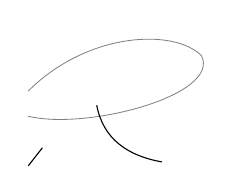
\begin{tikzpicture}[x=1cm,y=1cm,baseline=0pt]\draw[gray,line width=0.3pt] (-0.15,0.10) .. controls (0.60,0.85) and (1.70,0.90) .. (2.05,0.55) .. controls (2.30,0.05) and (0.60,-0.40) .. (-0.15,-0.22);\draw (-0.15,-0.85)--(0.03,-0.62);\draw (0.72,-0.08) .. controls (0.80,-0.5) and (1.1,-0.72) .. (1.55,-0.8);\end{tikzpicture}}\handwritten{pas prouvé}}
\uline{Corollaire} 7.3. \inserted{(Si $n$ pair\inserted{\handwritten{$\geq4$,}}, $X$ lisse).} On peut trouver un ouvert $U'$ \inserted{\handwritten{(non vide de la grassmannienne des droites)\deleted{de}}} de $S_d$, tel que pour toute droite \inserted{\handwritten{$D\in U'(k')$}\rlap{\begin{tikzpicture}[baseline]\draw (.1em,.2em) circle (.1em);\draw (.17em,.28em)--(.6em,1em);\end{tikzpicture}}} de $\handwritten{(}S_d\handwritten{)_{k'}}$ \deleted{qui, rencontre un $\unsure{U|U'}_{\handwritten{\unsure{k'|k}}}$ et qui définit}\inserted{\handwritten{$D$ est}} un pinceau de Lefschetz sur $X_{\handwritten{k'}}$, si $t$ désigne le point générique de cette droite, le motif $E(Y_t)$ des \deleted{\unsure{s}}cycles évanescents sur $Y_t$ \deleted{soit de} ne soit pas de niveau 1 (donc ne contienne pas de sous-motif $\handwritten{\ne}0$ de niveau 1, pas même sur une extension de $k(t)$, d'après le résultat de simplicité rappelé au n°6).
\margin{\handwritten{($k'$ une ext. \unsure{quele.|qqle.|quelc.} de $k$)}}

On prend $U$ comme dans la démonstration de 7.2, \inserted{\handwritten{et tel que les $Y_s$ $(s\in U)$ soient lisses.}\rlap{\begin{tikzpicture}[baseline]\draw (0,.8em) circle (.12em);\draw (0,.68em)--(-.2em,0);\end{tikzpicture}}} On peut (grâce au fait qu'un motif de niveau $\handwritten{\leq}\deleted{\unsure{\leq|<}}1$ se spécialise en un motif de niveau $\handwritten{\leq}1$, comme on a signalé au n°6 comme conséquence du critère de Ogg-Néron-Chafarévitch) supposer que $k$ est fini, et \unsure{\deleted{on}il|\deleted{il}on} \deleted{est ramené à prouver que} suffit de prouver que l'on peut trouver un point fermé $s$ de $D\handwritten{\cap U}$ tel que les valeurs propres de Frobenius opérant sur $E^{n-1}.(Y_s,\underline{Q}_{\handwritten{\ell}})$ ($\handwritten{\ell}$ un nombre premier fixé $\handwritten{\ne\ell}$) ne soient pas toutes divisibles par $p$. Or le nombre de points de $Y_t$ est égal à la somme alternée des traces de frobenius opérant sur les \deleted{\handwritten{$\unsure{H|E}_t^i$}}
\margin{\rlap{\begin{tikzpicture}[x=1cm,y=1cm,baseline=0pt]\draw (-0.13,0.24) .. controls (-0.32,0.16) and (-0.20,-0.05) .. (-0.18,-0.25) -- (-0.12,-2.35) .. controls (-0.10,-2.60) and (0.15,-2.66) .. (0.45,-2.60) -- (12.65,-2.50) .. controls (12.96,-2.47) and (13.12,-2.35) .. (13.08,-2.03) -- (13.02,-1.28);\draw (13.02,-1.23) -- (12.98,0.17) .. controls (12.95,0.38) and (12.80,0.46) .. (12.55,0.43) -- (0.22,0.38) -- (-0.13,0.24);\draw[gray,line width=0.3pt] (8.0,-2.85) .. controls (10.0,-2.80) and (12.0,-2.83) .. (13.45,-2.95);\draw (-0.38,0.20) circle (0.045);\draw (-0.40,0.17)--(-0.65,-0.28);\end{tikzpicture}}\parbox[t]{13cm}{\handwritten{$U'$ est défini comme \unsure{l'ouvert} de droites \inserted{$D$} rencontrant $U$ et telles que $\pi_1(\overline{D\cap U})\longrightarrow\pi_1(\bar U)$ soit surjectif (le $\bar{\phantom{k}}$ désigne \unsure{passage|pass.} à $\bar{k}'$). On utilise une variante \unsure{convenable} de Bertini}}}
% archive sheet number: 19
